\documentclass{article}
\usepackage{graphicx}

\title{Short Encounters at JMM 2023}
\author{Edward Yu}

\begin{document}

\maketitle
This year’s Joint Mathematics Meetings—the largest gathering of mathematicians in the United States—was hosted in Boston, MA. It usually attracts between 5,000 and 6,000 mathematicians from all walks of life, in all stages of their careers. This year, some high school students from the Seattle area (including me and Competitions Committee Director Alex Z.) had the exciting opportunity to attend this year’s Joint Mathematics Meetings through a math research program.

\begin{center}
    \footnotesize
    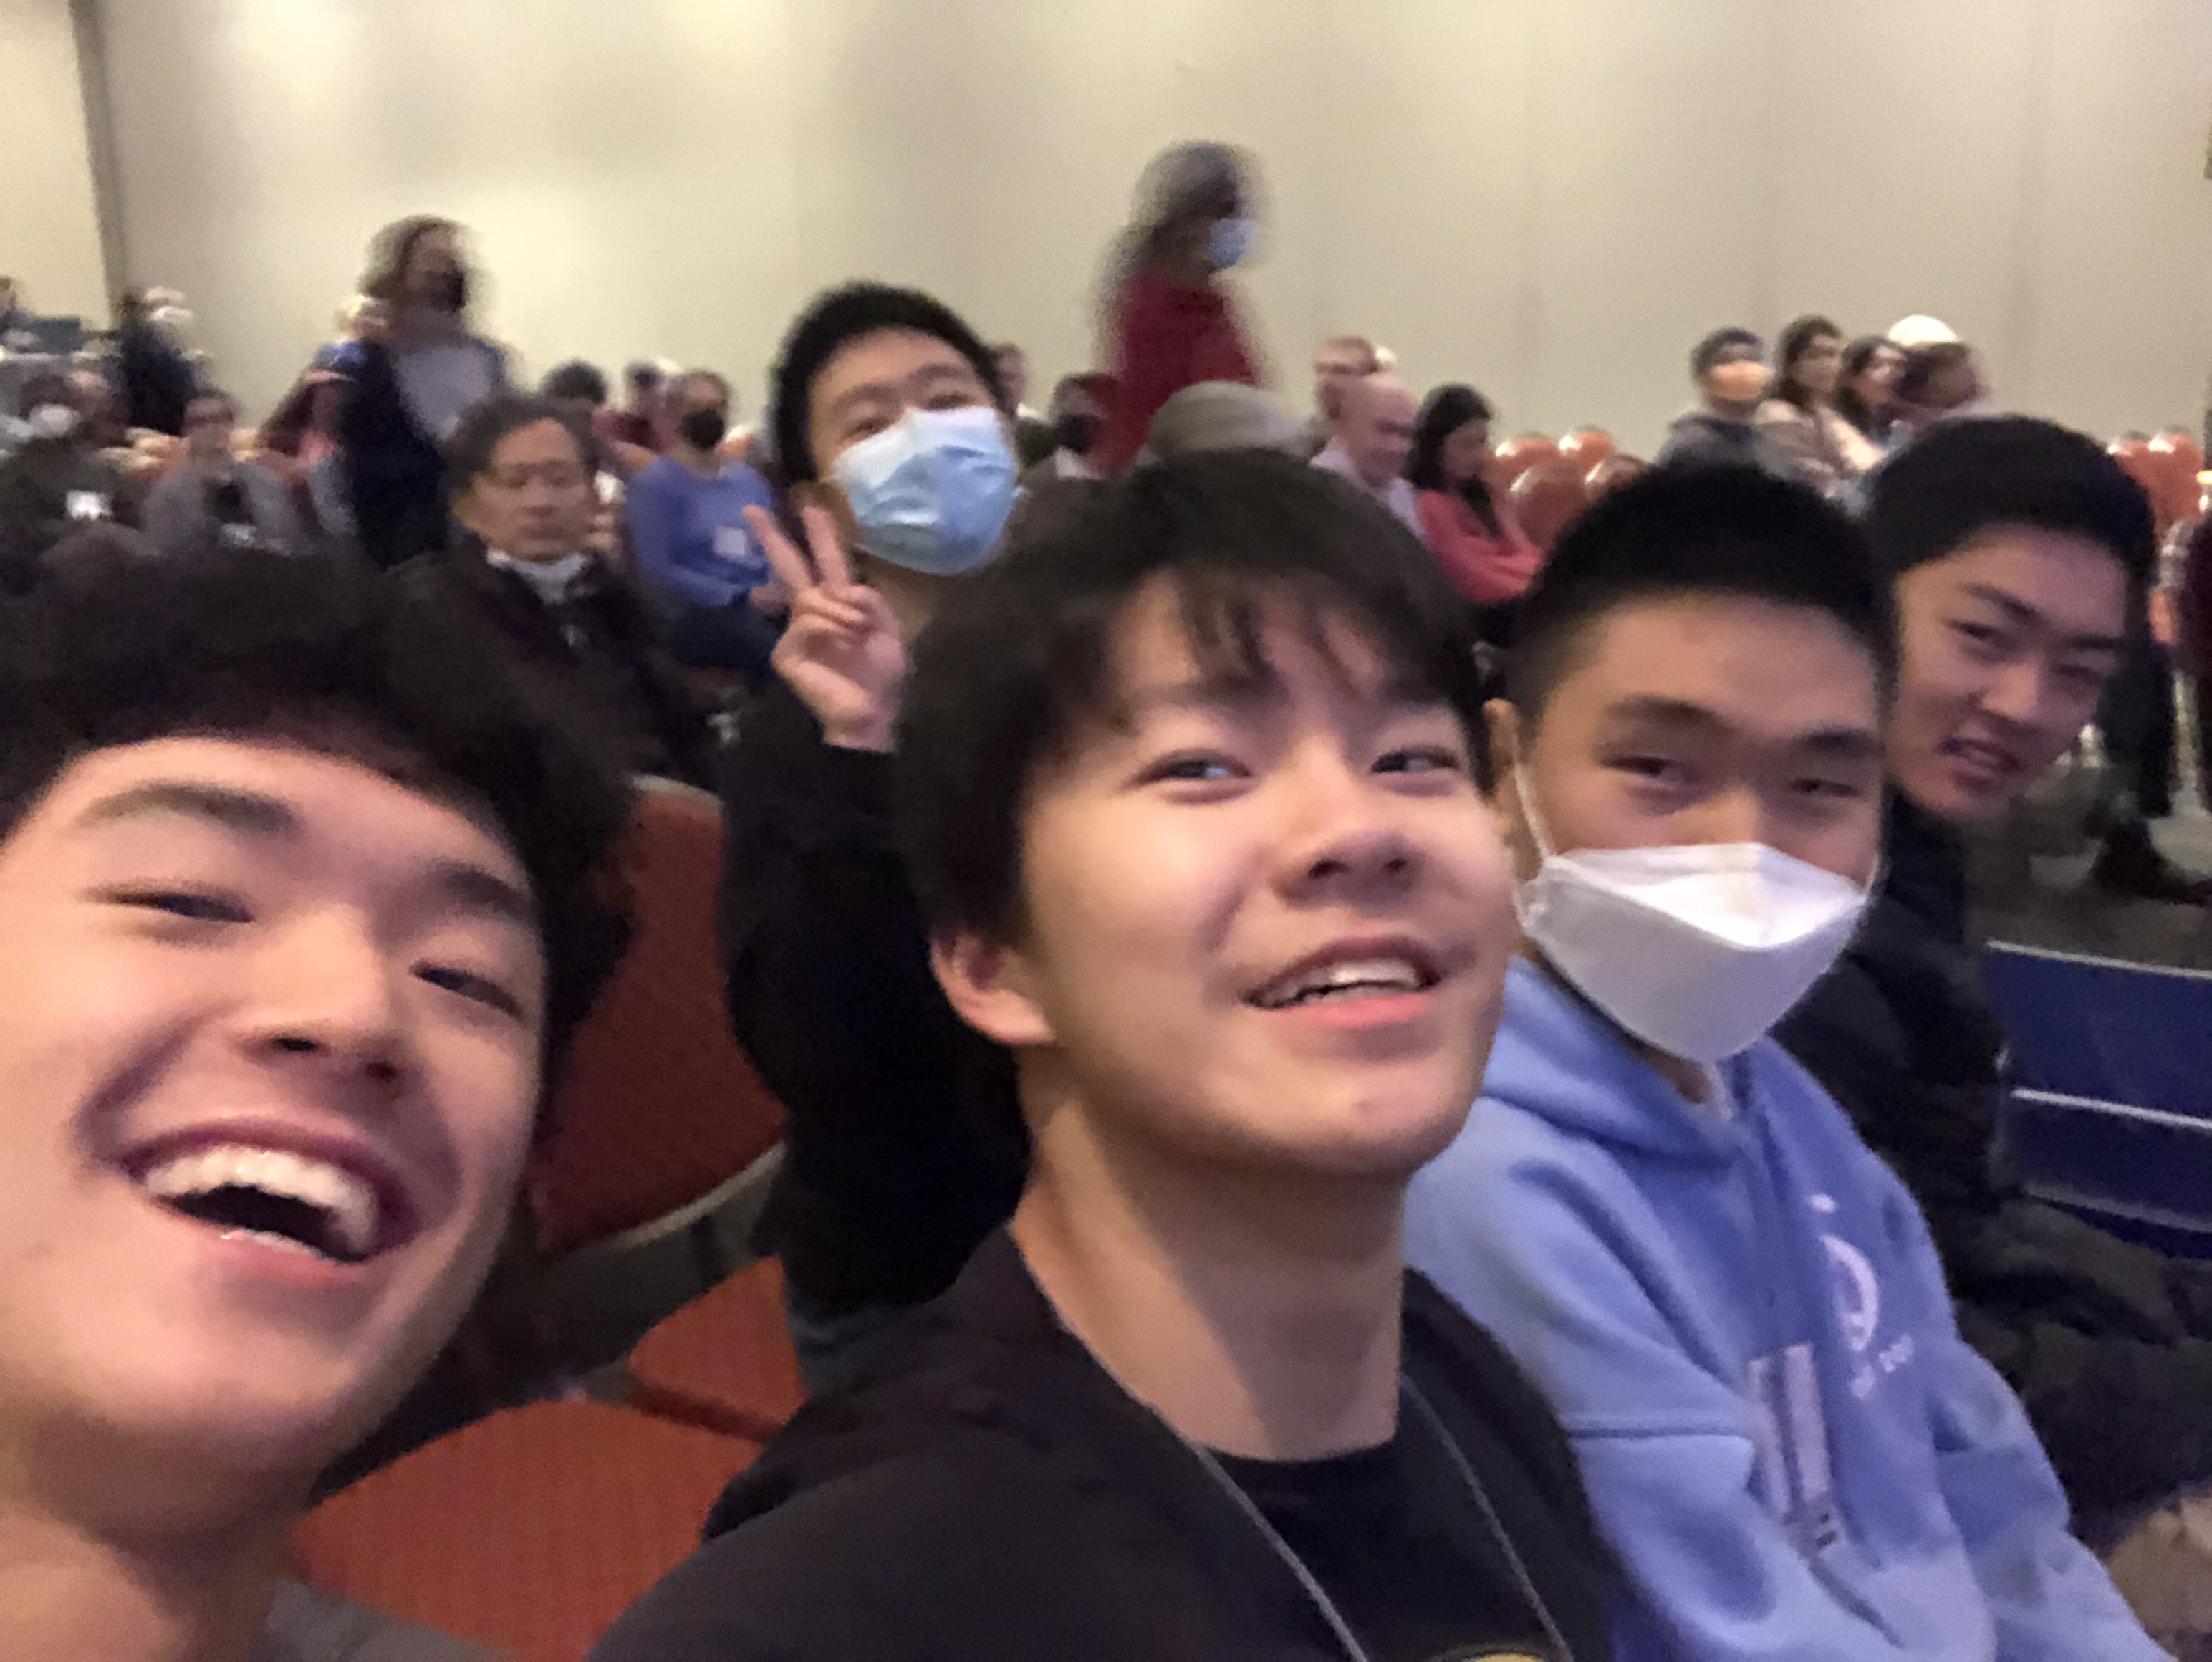
\includegraphics[scale = 0.04]{images/alexetal.png}
    
    President Edward Y. and Competitions Committee Director Alex Z. posing for a photo at JMM!
\end{center}

I had a few memorable encounters at JMM to share.

A talk by Grant Sanderson (known for his \href{https://www.youtube.com/@3blue1brown}{YouTube channel 3Blue1Brown}), who was a recipient of this year’s JPBM Communications Award. His, titled “Raising the Ceiling and Lowering the Floor of Math Exposition,” focused on how to deliver math content to students in a way that optimizes for understanding, rather than perfect rigor. One of his main points was that students learn more when they figure things out for themselves, and they learn less when shown the most beautiful, elegant proof without having struggled themselves. Next time when you feel frustrated while solving a difficult problem, don’t give up, and bang your head on the table for just a little longer! I’m joking, of course, but there is a grain of truth in there.

\begin{center}
    \footnotesize
    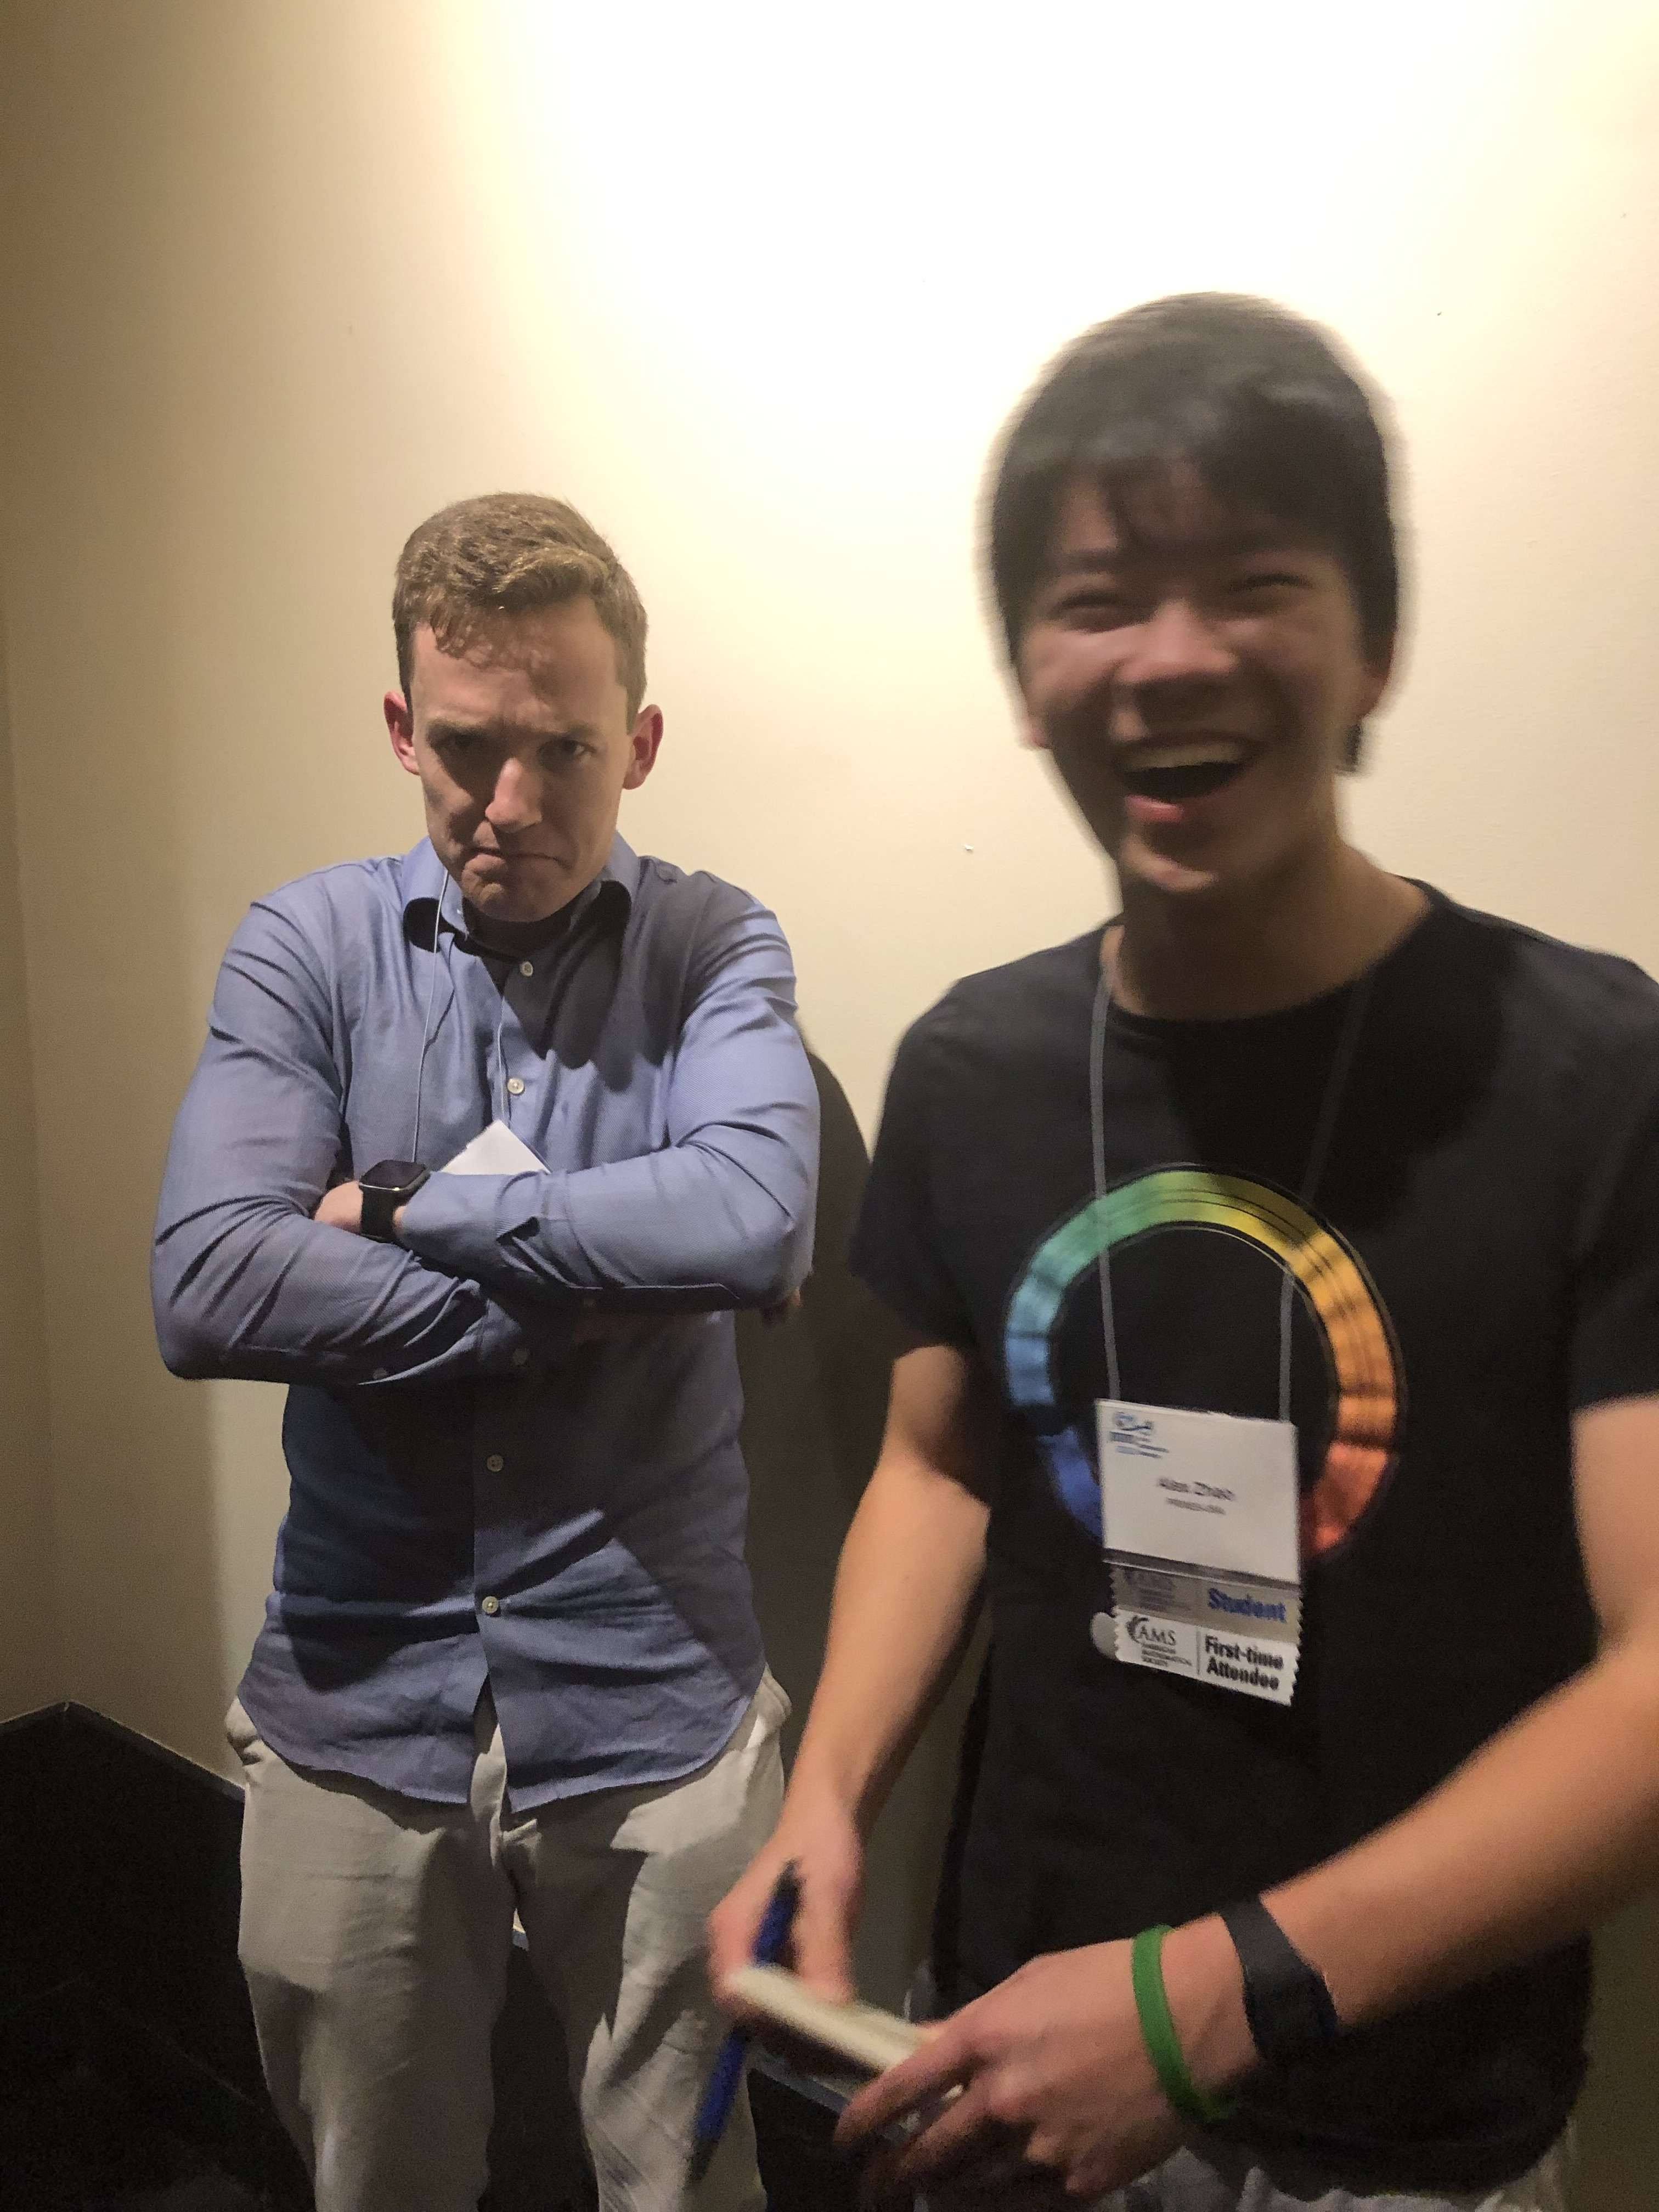
\includegraphics[scale = 0.045]{images/grantangry.png}
    
    Competitions Committee Director Alex Z. posing with an ``angry" Grant Sanderson.
\end{center}

A talk by Jordan Ellenberg (known for his books \textit{How Not to Be Wrong}, and more recently \textit{Shape}), the other recipient of the JPBM Communications Award. His talk, on “Outward-facing Mathematics,” was about how to write about mathematics for a general audience without boring them or scaring them away. To quote Jordan himself: “Yes, you’re really excited about Lemma 6.24, but please do not write your news article about Lemma 6.24.” Instead, he says, we should emphasize that mathematics is a human activity carried out by human beings for human purposes. So-called “dumbing down” the content is unnecessary and condescending, but judicious pruning helps keep content engaging.

At a talk titled “Partitioning Consecutive Powers into Sets of Equal Sum,” the speaker, Enrique Treviño, opened by saying: “this talk generalizes a puzzle by Dean Ballard in the 538 Riddler…” This was a highly interesting moment: some of you in the Seattle area may know Mr. Ballard as the long-time math coach at Lakeside School, who, besides helping facilitate math events at the school, also frequently sends intriguing puzzles to his students. In case you are curious, the puzzle is the “Riddler Classic” about spheres, here: \href{https://fivethirtyeight.com/features/can-you-flip-the-magic-coin/}{https://fivethirtyeight.com/features/can-you-flip-the-magic-coin/}. 

Glimpsing a celebrity is a surreal experience. Imagine my surprise when, during a lecture in a fully-packed meeting room, I looked at the person standing to my right and saw their name badge — Francis Su, former president of the Mathematical Association of America and current Vice President of the American Mathematical Society!

Want to catch some mathematics celebrities, and listen to some fascinating mathematical talks yourself? You can catch JMM 2024 in San Francisco, or, if you have a little more patience, wait for JMM to come to you in Seattle. Long story short, JMM 2022 was originally planned to be in Seattle, but switched to virtual programming with the onset of the Omicron variant of COVID-19. This unfortunate occurrence brings a silver lining for the future: JMM 2025 is scheduled for January 8-11, to be hosted in Seattle once more. Time to mark your calendars, and see you all in January 2025…
\end{document}